\documentclass[]{beamer}
%uncomment for notes
%\documentclass[handout]{beamer}
%\setbeameroption{show notes}
%\usepackage{pgfpages}
%\pgfpagesuselayout{4 on 1}[a4paper,border shrink=5mm,landscape]

\graphicspath{{output/}{resources/}}
\DeclareGraphicsExtensions{.pdf,.jpeg,.png,.jpg}
\usepackage[utf8]{inputenc}
\usepackage{epstopdf}
\usepackage{subcaption}
\usepackage{amsmath}
\usepackage{amssymb}
\usepackage{svg}
\usepackage[round]{natbib}
\usepackage{tikz}
\usetikzlibrary{fit}
\usetikzlibrary{arrows}
\usetikzlibrary{positioning}

\title{QSAR biodegradation dataset classification using neural networks}
\author{Jonáš Kulhánek, Jan Uhlík}
\institute{MFF, Charles University in Prague}
\date{December 2019}

\usepackage{natbib}
\usepackage{graphicx}
\setbeamertemplate{footline}[frame number]
\setbeamercolor{footline}{fg=blue}
\setbeamerfont{footline}{series=\bfseries}

\begin{document}
	\frame[noframenumbering,plain]{
		\titlepage
	}
	\frame {
    \frametitle{QSAR biodegradation dataset\cite{dataset}}
		\begin{itemize}
        \item classification dataset where the task is to predict whether a protein is bio-degradable based on its chemical properties
		    \item published by Milano Chemometrics and QSAR Research Group
		    \item 41 attributes in total, some real valued, other integer valued
        \item number of proteins in the dataset is 1055
		\end{itemize}
	}
	
	\frame{
	    \frametitle{Outline}
	    \begin{itemize}
	        \item 3D environment simulators
	        \item base algorithm
	           \note{\textbf{base algorithm} \\ \hspace{2em}algorithm based on a2c, a3c will be discussed with improvements \\}
	        \item our method
	            \note{\textbf{our method} \\ \hspace{2em}improve on the base algorithm, discuss the network architecture \\}
	        \item experiments
	            \note{\textbf{experiments} \\ \hspace{2em}experiments we have done will be presented \\}
	        \item conclusions \& future work
	            \note{\textbf{conclusions \& future work} \\ \hspace{2em}discussion, quality of this method, future work \\}
	    \end{itemize}
	}

  \frame{
    \frametitle{Single layer network training}
    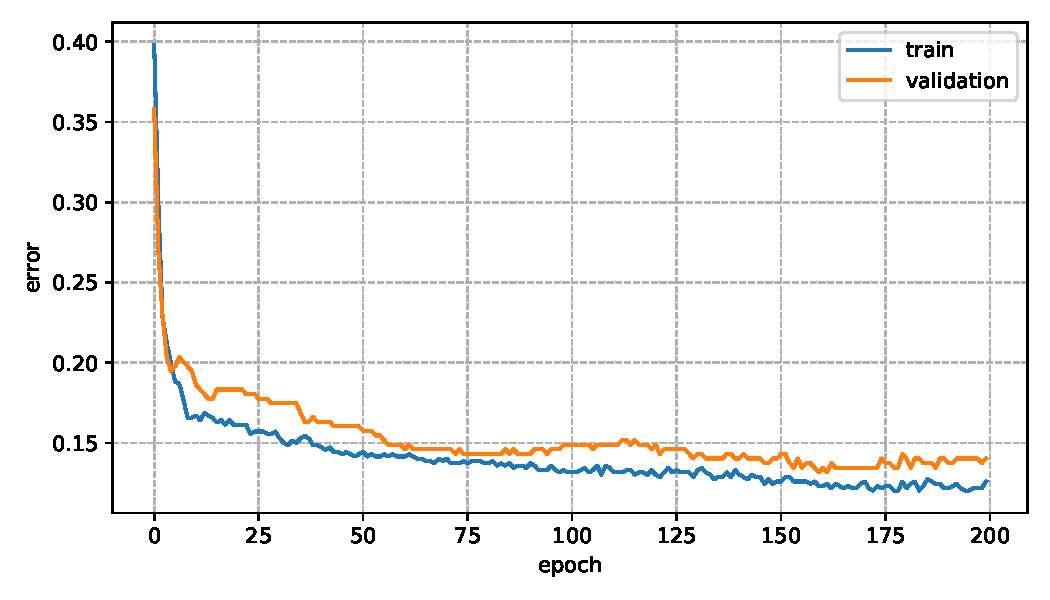
\includegraphics[width=\linewidth]{logreg}
  }

	\frame{
    \cite{*}
    	\bibliographystyle{plainnat}
        \bibliography{references}
	}
	
  \end{document}	
